\section{Título de la Segunda sección}
Contenido de la segunda sección. Primera bibliografia:\cite{bib2}


\subsection{Título de la primera subsección}
Contenido de la primer subsección. La figura 1 es un ejemplo de una Figura \ref{imagen2}.

\begin{figure}[h] %Ambiente para figuras, here.
    \begin{center}
        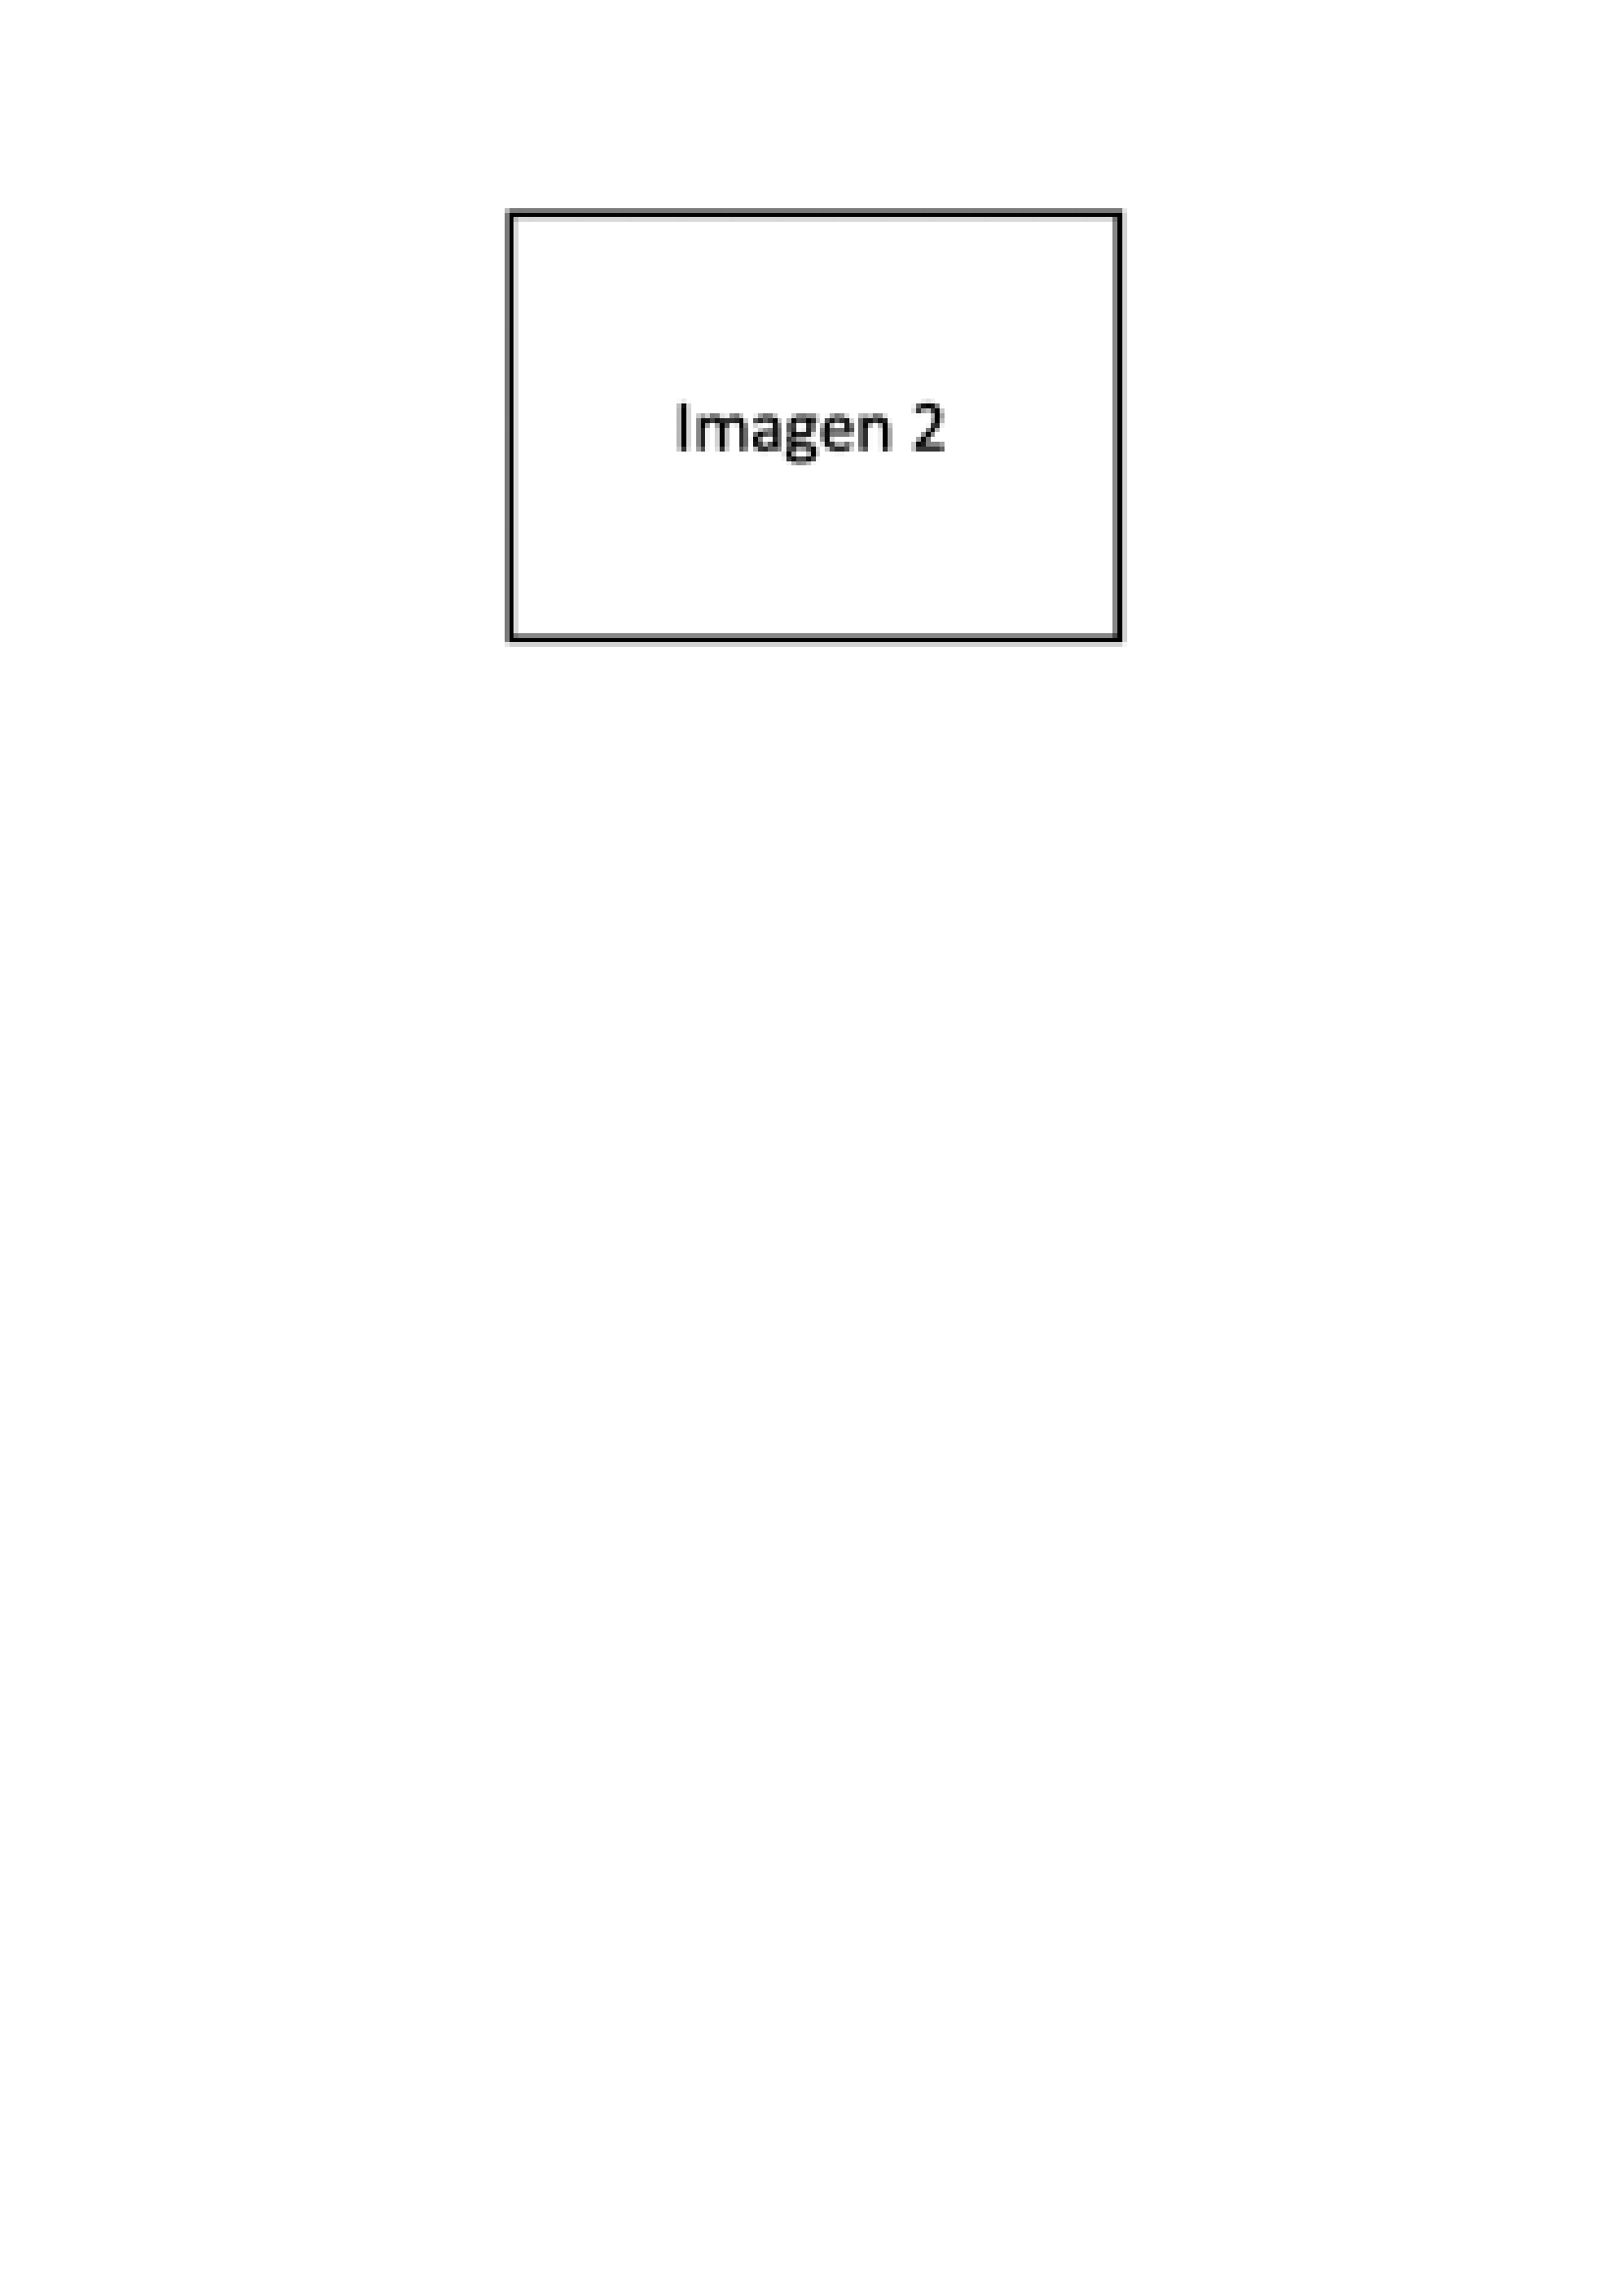
\includegraphics[scale=0.20]{secciones/imagenes/imagen2.png}
    \end{center}
    \caption{Ejemplo de figura. \label{imagen2}}
\end{figure}

\subsection{Título de la segunda subsección}
Contenido de la segunda subsección. Ejemplo de ecuación matemática es la ecuación 1:

\begin{equation}
    e=mc^2
    \label{ecuacion}
\end{equation}
Así se escribe la chicharronera: $x = \frac {-b \pm \sqrt {b^2 - 4ac}}{2a}$ 

\subsection{Título de la tercera subsección}
Contenido de la tercera subsección. A continuación se muestra un ejemplo de elementos en viñetas:

\begin{itemize} %ambiente o entorno itemize
    \item [+]\textit{uno.}
    \item \textbf{dos.}
    \item \underline{tres.}
    \item cuatro.
\end{itemize}


